%! suppress = MissingImport
%%
%% DuplicatorLab (c) 22 Christopher A. Bohn
%%
%% Licensed under the Apache License, Version 2.0 (the "License");
%% you may not use this file except in compliance with the License.
%% You may obtain a copy of the License at
%%     http://www.apache.org/licenses/LICENSE-2.0
%% Unless required by applicable law or agreed to in writing, software
%% distributed under the License is distributed on an "AS IS" BASIS,
%% WITHOUT WARRANTIES OR CONDITIONS OF ANY KIND, either express or implied.
%% See the License for the specific language governing permissions and
%% limitations under the License.
%%

%%
%% (c) 2021 Christopher A. Bohn
%%

\documentclass[12pt]{article}

\usepackage{fullpage}
\usepackage{fancyhdr}
\usepackage[procnames]{listings}
\usepackage{hyperref}
\usepackage{textcomp}
\usepackage{bold-extra}
\usepackage[dvipsnames]{xcolor}
\usepackage{etoolbox}


% Customize the semester (or quarter) and the course number

\newcommand{\courseterm}{Spring 2022}
\newcommand{\coursenumber}{CSCE 231}

% Customize how a typical lab will be managed;
% you can always use \renewcommand for one-offs

\newcommand{\runtimeenvironment}{your account on the \textit{csce.unl.edu} Linux server}
\newcommand{\filesource}{Canvas or {\footnotesize$\sim$}cse231 on \textit{csce.unl.edu}}
\newcommand{\filesubmission}{Canvas}

% These are placeholder commands and will be renewed in each lab

\newcommand{\labnumber}{}
\newcommand{\labname}{Lab \labnumber\ Assignment}
\newcommand{\shortlabname}{}
\newcommand{\duedate}{}

% Individual or team effort

\newcommand{\individualeffort}{This is an individual-effort project. You may discuss concepts and syntax with other students, but you may discuss solutions only with the professor and the TAs. Sharing code with or copying code from another student or the internet is prohibited.}
\newcommand{\teameffort}{This is a team-effort project. You may discuss concepts and syntax with other students, but you may discuss solutions only with your assigned partner(s), the professor, and the TAs. Sharing code with or copying code from a student who is not on your team, or from the internet, is prohibited.}
\newcommand{\freecollaboration}{In addition to the professor and the TAs, you may freely seek help on this assignment from other students.}
\newcommand{\collaborationrules}{}

% Do you care about software engineering?

\providebool{allowspaghetticode}

\setbool{allowspaghetticode}{false}

\newcommand{\softwareengineeringfrontmatter}{
    \ifboolexpe{not bool{allowspaghetticode}}{
        \section*{No Spaghetti Code Allowed}
        In the interest of keeping your code readable, you may \textit{not} use
        any \lstinline{goto} statements, nor may you use any \lstinline{break}
        statements to exit from a loop, nor may you have any functions
        \lstinline{return} from within a loop.
    }{}
}

\newcommand{\spaghetticodepenalties}[1]{
    \ifboolexpe{not bool{allowspaghetticode}}{
        \penaltyitem{1}{for each \lstinline{goto} statement, \lstinline{break}
            statement used to exit from a loop, or \lstinline{return} statement
            that occurs within a loop.}
    }{}
}

% You shouldn't need to customize these,
% but you can if you like

\lstset{language=C, tabsize=4, upquote=true, basicstyle=\ttfamily}
\newcommand{\function}[1]{\textbf{\lstinline{#1}}}
\setlength{\headsep}{0.7cm}
\hypersetup{colorlinks=true}

\newcommand{\startdocument}{
    \pagestyle{fancy}
    \fancyhf{}
    \lhead{\coursenumber}
    \chead{\ Lab \labnumber: \labname}
    \rhead{\courseterm}
    \cfoot{\shortlabname-\thepage}

	\begin{document}
	\title{\ Lab \labnumber}
	\author{\labname}
	\date{Due: \duedate}
	\maketitle

    \textit{\collaborationrules}
}

\newcommand{\rubricitem}[2]{\item[\underline{\hspace{1cm}} +#1] #2}
\newcommand{\bonusitem}[2]{\item[\underline{\hspace{1cm}} Bonus +#1] #2}
\newcommand{\penaltyitem}[2]{\item[\underline{\hspace{1cm}} -#1] #2}

%%
%% labs/common/semester.tex
%% (c) 2021-22 Christopher A. Bohn
%%
%% Licensed under the Apache License, Version 2.0 (the "License");
%% you may not use this file except in compliance with the License.
%% You may obtain a copy of the License at
%%     http://www.apache.org/licenses/LICENSE-2.0
%% Unless required by applicable law or agreed to in writing, software
%% distributed under the License is distributed on an "AS IS" BASIS,
%% WITHOUT WARRANTIES OR CONDITIONS OF ANY KIND, either express or implied.
%% See the License for the specific language governing permissions and
%% limitations under the License.
%%


% Customize the semester (or quarter) and the course number

\newcommand{\courseterm}{Fall 2022}
\newcommand{\coursenumber}{CSCE 231}

% Customize how a typical lab will be managed;
% you can always use \renewcommand for one-offs

\newcommand{\runtimeenvironment}{your account on the \textit{csce.unl.edu} Linux server}
\newcommand{\filesource}{Canvas or {\footnotesize$\sim$}cse231 on \textit{csce.unl.edu}}
\newcommand{\filesubmission}{Canvas}

% Customize for the I/O lab hardware

\newcommand{\developmentboard}{Arduino Nano}
%\newcommand{\serialprotocol}{SPI}
\newcommand{\serialprotocol}{I2C}
%\newcommand{\displaymodule}{MAX7219digits}
%\newcommand{\displaymodule}{MAX7219matrix}
\newcommand{\displaymodule}{LCD1602}

\setbool{usedisplayfont}{true}

\newcommand{\obtaininghardware}{
    The EE Shop has prepared ``class kits'' for CSCE 231; your class kit costs \$30.
    The EE Shop is located at 122 Scott Engineering Center and is open M-F 7am-4pm. You do not need an appointment.
    You may pay at the window with cash, with a personal check, or with your NCard.
    The EE shop does \textit{not} accept credit cards.
}

% Update to reflect the CS2 course(s) at your institute

\newcommand{\cstwo}{CSCE~156, RAIK~184H, or SOFT~161}

% Do you care about software engineering?

\setbool{allowspaghetticode}{false}

% Which assignments are you using this semester, and when are they due?

\newcommand{\pokerlabnumber}{1}
\newcommand{\pokerlabcollaboration}{
    Sections~\ref{sec:connecting}, \ref{sec:terminology}, \ref{sec:gettingstarted}, \ref{subsec:typesofpokerhands}, and~\ref{subsec:studythecode}: \freecollaboration
    Sections~\ref{sec:completingcard} and~\ref{subsec:completepoker}: \individualeffort
}
\newcommand{\pokerlabdue}{Week of August 29, before the start of your lab section}

\newcommand{\keyboardlabnumber}{2}
\newcommand{\keyboardlabcollaboration}{\individualeffort}
\newcommand{\keyboardlabdue}{Week of January 31, before the start of your lab section}

\newcommand{\pointerlabnumber}{3}
\newcommand{\pointerlabcollaboration}{\individualeffort}
\newcommand{\pointerlabdue}{Week of February 7, before the start of your lab section}

\newcommand{\integerlabnumber}{4}
\newcommand{\integerlabcollaboration}{\individualeffort}
\newcommand{\integerlabdue}{Week of February 14, before the start of your lab section}

\newcommand{\floatlabnumber}{5}
\newcommand{\floatlabcollaboration}{\individualeffort}
\newcommand{\floatlabdue}{soon}

\newcommand{\addressinglabnumber}{6}
\newcommand{\addressinglabcollaboration}{\individualeffort}
\newcommand{\addressinglabdue}{Week of February 28, before the start of your lab section}

%bomblab was 7
%attacklab was 8

\newcommand{\pollinglabnumber}{9}
\newcommand{\pollinglabcollaboration}{\individualeffort}
\newcommand{\pollinglabdue}{Week of April 11, before the start of your lab section}
\newcommand{\pollinglabenvironment}{your \developmentboard-based class hardware kit}

\newcommand{\ioprelabnumber}{\pollinglabnumber-prelab}
\newcommand{\ioprelabcollaboration}{\freecollaboration}
\newcommand{\ioprelabdue}{Before the start of your lab section on April 5 or 6}

\newcommand{\interruptlabnumber}{10}
\newcommand{\interruptlabcollaboration}{\individualeffort}
\newcommand{\interruptlabdue}{Week of April 18, before the start of your lab section}
\newcommand{\interruptlabenvironment}{your \developmentboard-based class hardware kit}

\newcommand{\capstonelab}{ComboLock}    % this will come into play when we generalize capstonelab
\newcommand{\capstonelabnumber}{11}
\newcommand{\capstonelabcollaboration}{\teameffort}
\newcommand{\capstonelabdue}{Week of May 2, Before the start of your lab section\footnote{See Piazza for the due dates of teams with students from different lab sections.}}
\newcommand{\capstonelabenvironment}{your \developmentboard-based class hardware kit}

\newcommand{\memorylabnumber}{12}
\newcommand{\memorylabcollaboration}{This is an individual-effort project. You may discuss the nature of memory technologies and of memory hierarchies with classmates, but you must draw your own conclusions.}
\newcommand{\memorylabdue}{Week of May 2, at the end of your lab section}
\newcommand{\memorylabenvironment}{your \developmentboard-based class hardware kit and your account on the \textit{csce.unl.edu} Linux server}

% Labs not used this semester

\newcommand{\concurrencylabnumber}{XX}
\newcommand{\concurrencylabcollaboration}{\individualeffort}
\newcommand{\concurrencylabdue}{not this semester}

\newcommand{\ssbcwarmupnumber}{XX}
\newcommand{\ssbcwarmupcollaboration}{\freecollaboration}
\newcommand{\ssbcwarmupdue}{not this semester}

\newcommand{\ssbcpollingnumber}{XX}
\newcommand{\ssbcpollingcollaboration}{\individualeffort}
\newcommand{\ssbcpollingdue}{not this semester}

\newcommand{\ssbcinterruptnumber}{XX}
\newcommand{\ssbcinterruptcollaboration}{\individualeffort}
\newcommand{\ssbcinterruptdue}{not this semester}

%%
%% labs/common/storylines.tex
%% (c) 2020-23 Christopher A. Bohn
%%
%% Licensed under the Apache License, Version 2.0 (the "License");
%% you may not use this file except in compliance with the License.
%% You may obtain a copy of the License at
%%     http://www.apache.org/licenses/LICENSE-2.0
%% Unless required by applicable law or agreed to in writing, software
%% distributed under the License is distributed on an "AS IS" BASIS,
%% WITHOUT WARRANTIES OR CONDITIONS OF ANY KIND, either express or implied.
%% See the License for the specific language governing permissions and
%% limitations under the License.
%%

\newcommand{\MeetArchie}{
    \begin{wrapfigure}{r}{0.33\textwidth}
        \centering
        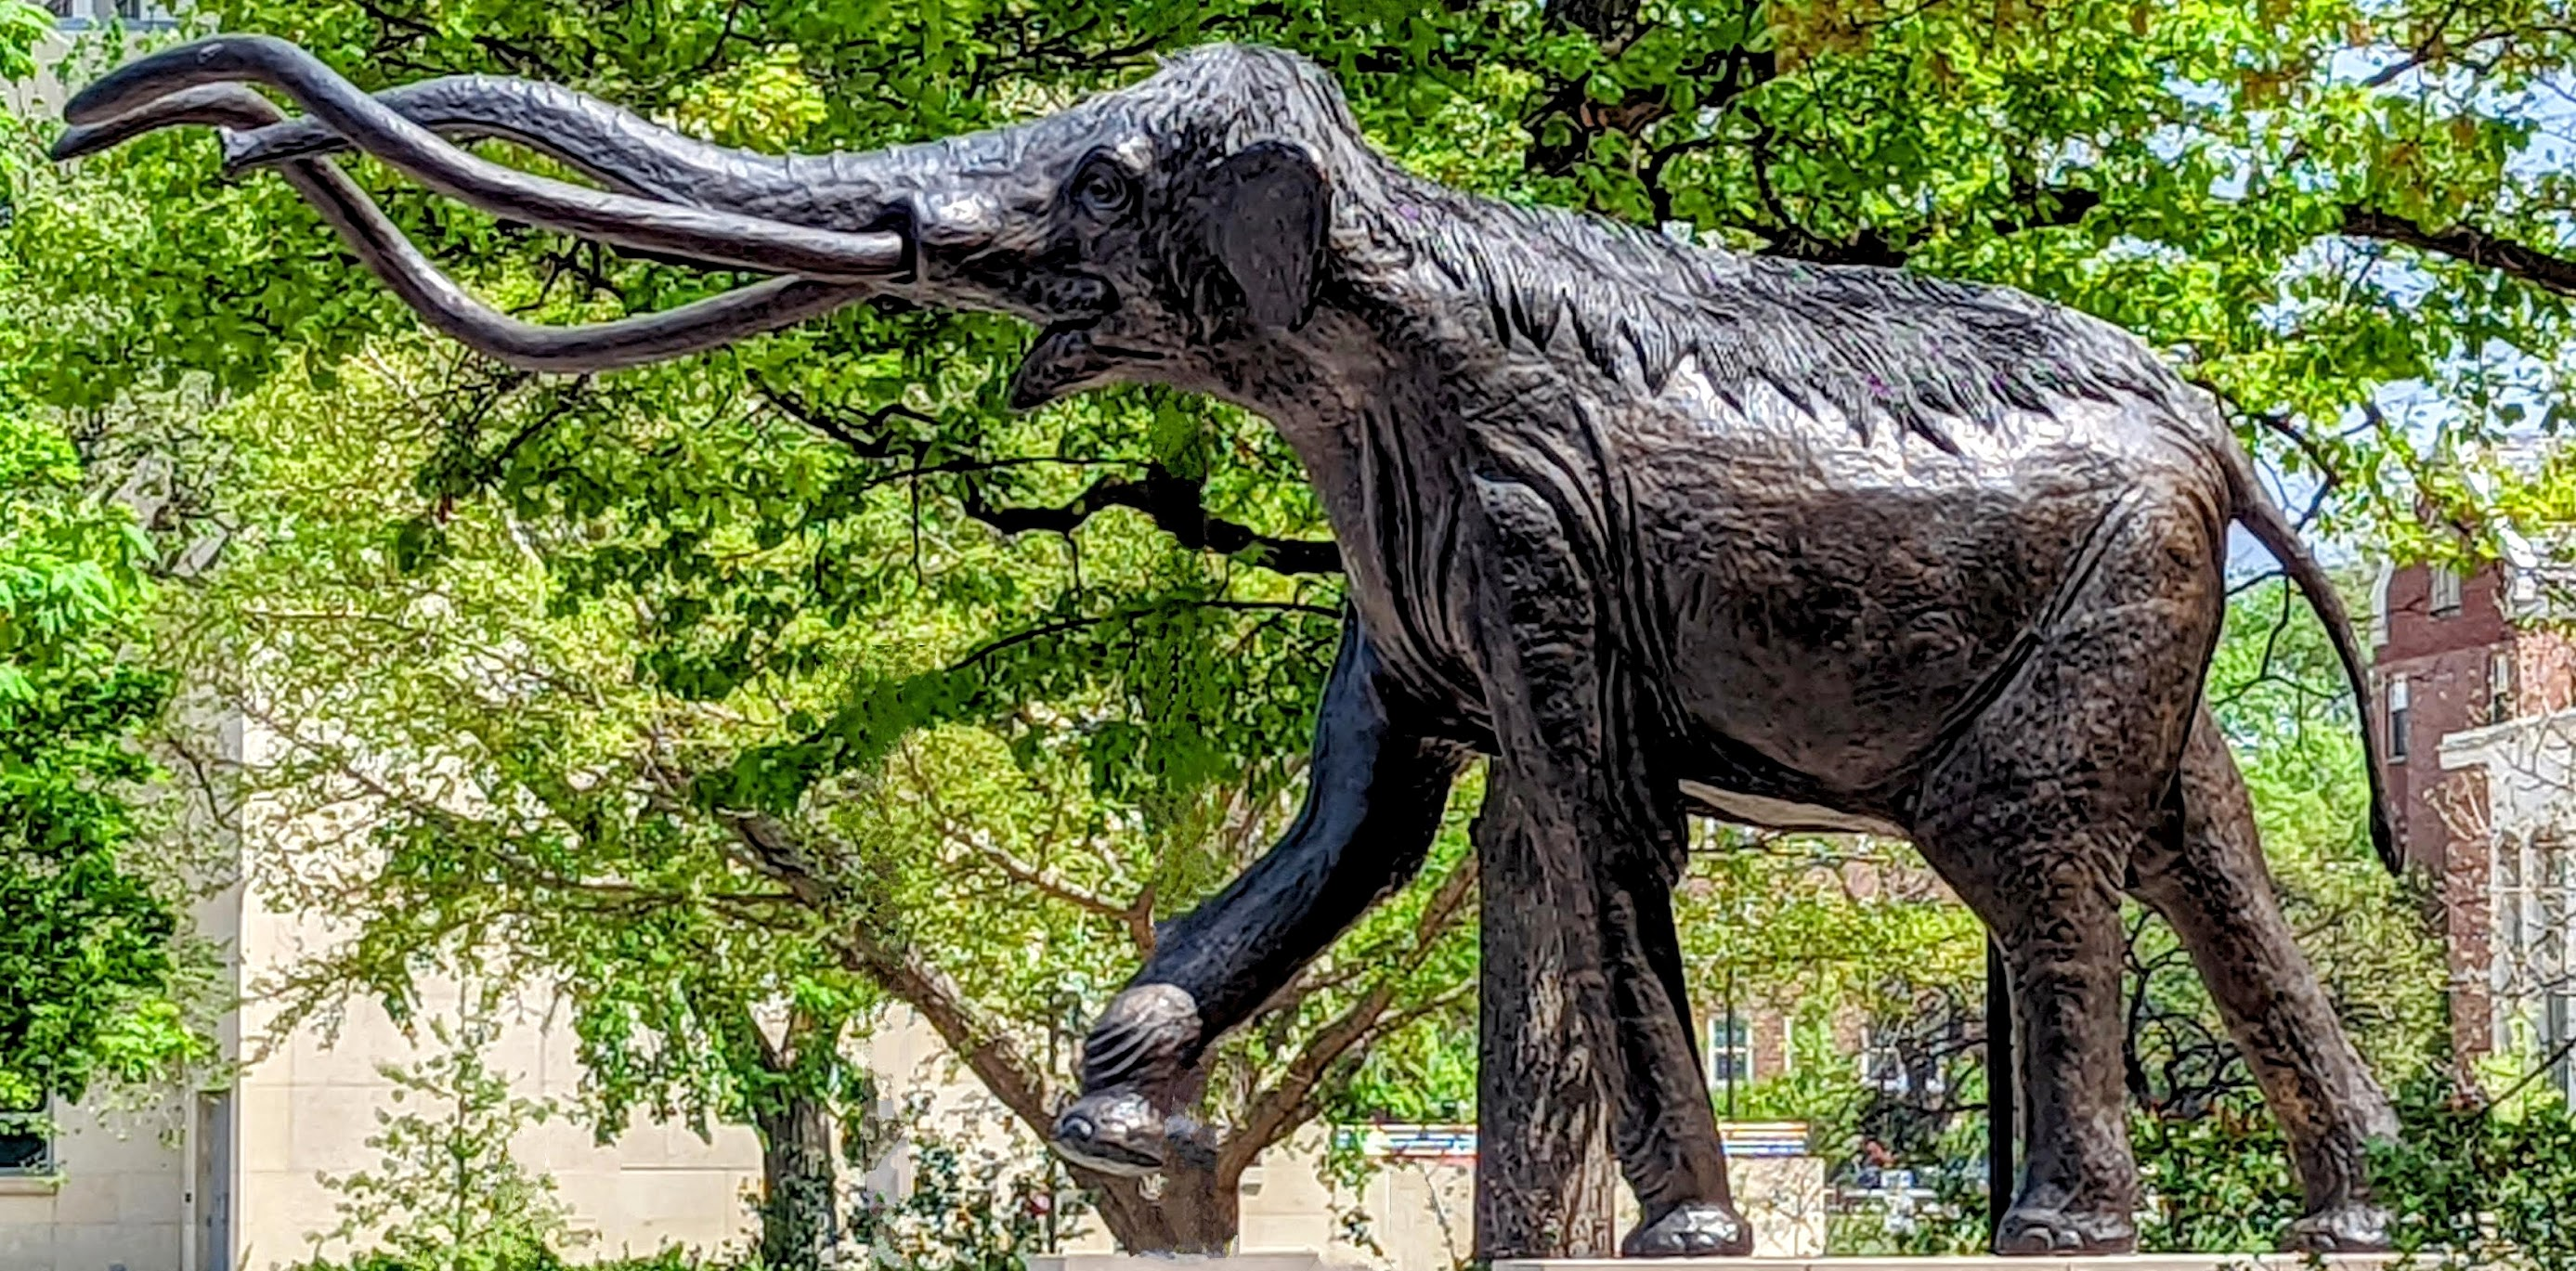
\includegraphics[width=.4\textwidth]{archie}
        \caption{Archie.\\ \footnotesize{Photograph by Bohn.}}
    \end{wrapfigure}

    You're relaxing at your favorite hangout when another customer catches your attention.
    He's rather large (dare I say, \textit{mammoth}), a bit hairy, and looking frustrated in front of his laptop.
    ``I'm Archie,'' he says, ``and I'm trying to teach myself this card game called \textit{Poker}.
    I found this source code that I thought I could use to understand Poker better, but the code is incomplete, and I don't entirely understand what's there.
    Could you explain the code to me, please?'
}

\newcommand{\GetHired}{
    Archie's face lights up in a very big smile.
    ``Thanks!''
    After pausing in thought for a moment, he says, ``Say, I've got a new startup company that could really use your help.
    Are you interested?
    It'll be exciting!''
}

\newcommand{\FirstDayOnTheJob}{
    \begin{wrapfigure}{r}{0.33\textwidth}
        \centering
        
\includegraphics[width=.4\textwidth]{some-expenses-spared}
        \caption{Some expenses were spared.\\ \footnotesize{Original images \textcopyright\ Universal Studios and Amblin Entertainment, Inc. Meme creator unknown.}}
    \end{wrapfigure}

    You've recently been hired to help get the Pleistocene Petting Zoo get started.
    Your new employer, Archie, is surprisingly honest: he admits to you that some expenses were spared.
    Archie cheerfully points out that any challenge is also an opportunity to succeed.
    You suspect your job will offer plenty of ``opportunities to succeed.''
}

\newcommand{\HasKeyboard}{
    Great news!
    Archie brings you your new keyboard.
    He also brings you a problem of his own.
    Because you were held up with the broken keyboard, Archie decided to try some programming on his own, and his code is behaving strangely.
}

\newcommand{\ArchieWroteSmellyCode}{
    Working at the Pleistocene Petting Zoo certainly is proving to be interesting.
    You're glad that you don't have to worry about the problem of the giant sloths very slowly chasing their handlers, but now it seems that Archie has decided to try to write a program or two.
    At a glance, his code is smellier than the wooly rhinoceros' enclosure.
    But you take a closer look anyway to try to understand why his code acts strangely.
}

\newcommand{\InsurancePreview}{
    You hear somebody enter the room.
    ``\textit{Frankenstein}, `boat','' is the challenge, and she answers, ``borne.''
    Archie introduces you to the new arrival, ``Lil, this is our new developer, the one who wrote the app we just used.''
    He turns to you: ``This is Lilith Redd from business operations.''
    He turns back to her and continues, ``Lil, what's the good word?''

    ``The word isn't good, I'm afraid.
    I just heard back from the insurance company.''
}

\newcommand{\OnLoanToEclecticElectronics}{
    All work at the Pleistocene Petting Zoo has stopped while Archie tries to find a $\cancelto{\mathrm{reasonable}}{\mathrm{gullible}}$ insurance company.
    Rather than furloughing staff, he's asked everybody to help out with his other startup companies for a week or two.
    He specifically asked that you help out with Eclectic Electronics.

    Herb Bee, the chief engineer, explains that Eclectic Electronics is developing a patent-pending C-licon tool that will convert C code into an integrated circuit that has the same functionality as the original C code.
    To test it out, he tasked you with writing the code to implement an Arithmetic Logic Unit (ALU).
    Your task will be to implement integer addition, subtraction, multiplication, and division.
    Even though high-level languages' \textit{logical} boolean operations normally are not part of an ALU, Herb wants you to include these in the ALU to see if that can make some programs run faster.
    Because bitwise operations and bit shift operations have been implemented, you will be able to use C's bitwise and bit shift operators, but because arithmetic operations have not yet been implemented, you cannot use C's arithmetic operators.
    Because C library functions generally make use of arithmetic operations (which have not yet been implemented), you cannot use library functions.
}

\newcommand{\SuccessfulALU}{
    Herb smiles as he hands you the the test results from the latest integrated circuit fab batch.
    ``C-licon successfully turned your code into an ALU.
    Nicely done!''
    I think maybe it's time to use C-licon to see if we can improve the Floating Point Unit (FPU) on our experimental microprocessor.
}

\newcommand{\WriteAnFPU}{
    Herb tells you that, Eclectic Electronics tested the integrated circuit that the C-licon tool created from your ALU code, and they've concluded that C-licon is ready to use for their new experimental microprocessor.
    He tasks you with writing C code (that will be used by the C-licon tool) to implement a Floating Point Unit (FPU).
    Your task will be to implement floating point addition, subtraction, multiplication, and division.
    You can use any bit operations and, thanks to the ALU you wrote, you can use any integer arithmetic operations (use the conventional + - * / operators).
    Because the FPU has not yet been implemented, you cannot use C's floating point operations, you cannot use \lstinline{float}s nor \lstinline{double}s, and you cannot use library functions.
}

\newcommand{\GoingBackToTheZoo}{
    Lil enters the room.
    Herb challenges her: ``\textit{Gulliver's Travels}, `endian','' and Lil answers, ``ends.''

    Lil walks up to you and says, ``We have the insurance situation taken care of, and it's time to get the Zoo ready for guests.
    We're reassembling the tech team, and there's plenty of work to do.''

    You smile.
    ``That's good news!''

    Lil's face is hard to read.
    ``Well, yes and no.
    It's good that you'll be able to resume work on the Zoo's systems.
    But while Archie was waiting for us to fix the insurance situation, he got bored and -- cutting a long story short -- he ended up creating some new `opportunities' that we need you `to succeed' at.''
}

\newcommand{\SettledIntoRoutine}{
    You've settled into a comfortable routine at the Pleistocene Petting Zoo.
    While your job isn't quite as exciting as that of the saber-toothed tigers' dentist, it still has something new and interesting almost every day.

    Archie announces that he heard that hand-crafted assembly code can be faster than high-level language code.
    You try to explain that while this may have been true decades ago, modern optimizing compilers generate code faster than what a typical programmer can achieve with assembly code.
    Archie doesn't believe you and insists that you write the zoo's new cipher program in x86 assembly code.
}

\newcommand{\NewmanRanOffWithSamples}{
    Archie is hurriedly packing is trunk, like he's about to leave on a short-notice urgent trip.
    Before charging out the door, he pauses to tell you, ``Newman just stole some of our samples.
    I need to track him down before he sells them to the Supersized Safari Syndicate.
    I guess this means you're in charge of the Zoo's computer system now.
    Don't worry, you'll be fine. What could possibly go wrong?''
}

\newcommand{\BombLabIntroduction}{  % Ties Bryant & O'Halloran's Bomb Lab into the Pleistocene Petting Zoo story
    In a jarring collision of movie franchises, the CEO of Virtucon makes a Zoom call to the Pleistocene Petting Zoo.
    For some reason that nobody really explains, you're the only person available to handle the situation.
    The guy, who sounds kind of like an animated ogre, demands that the Pleistocene Petting Zoo deliver to him a megalodon shark with a head-mounted laser capable of emitting a beam of pure antimatter.

    You blurt out, ``Then it's not a laser,'' and then try to explain to him that megalodons are from the Miocene epoch, and expecting to find them at the Pleistocene Petting Zoo would be as ridiculous as a Cretaceous-period tyrannosaur at a Jurassic-themed park.

    ``Zip it!'' commands the guy who kind of looks like the host of a public-access show you used to watch.
    ``Since you won't meet my demand, my minions have placed a `binary bomb' under your zoo.
    Because I like really convoluted plans, we put software on your Linux server that controls the bomb.
    If you do nothing, the bomb will explode.
    If you turn off the Linux server, the bomb will explode.
    If you go slower than 50mph, the bomb will -- no, never mind that last part.

    ``The bomb software consists of a sequence of phases.
    Each phase expects you to type a particular string on \texttt{stdin}.
    If you type the correct string, then the phase is {\em defused} and the bomb proceeds to the next phase. Otherwise, the bomb {\em explodes}.
    The bomb is defused when every phase has been defused.

    ``Your mission, which you have no choice but to accept, is to defuse your bomb before the due date.
    Good luck, and welcome to the bomb squad!''
}

\newcommand{\FoodLockersAreStuck}{
    Having saved the Zoo from Dr. Evil's binary bomb, you relax back in your chair and think about taking a break.
%SPRINGBREAK
    Maybe an entire week in which you don't have solve any problems or meet any deadlines -- that'd be real nice.
%FALLBREAK
    % Maybe 4-day weekend in which you don't have solve any problems or meet any deadlines -- that'd be real nice.

    Another Zoom call comes in.
    \textit{What now!?} you wonder as you take your feet off of the desk to answer the call.
    An uncomfortable-looking animal handler says, ``We can't unlock the food lockers.
    It's the animals' feeding time, and we can't open the food lockers!
    It's feeding time, we can't get to the animals' food, and,'' his eyes dart nervously toward the animal enclosures, ``and many of them have sharp, pointy claws and others have big, stompy feet.''
}

\newcommand{\AttackLabIntroduction}{    % Ties Bryant & O'Halloran's Attack Lab into the Pleistocene Petting Zoo story
    You managed to keep the Pleistocene Petting Zoo from blowing to smithereens, but it turns out that Dr. Evil's minions weren't too careful when they put the bomb control software on the Zoo's Linux server.
    The software that controls the food locker has been heavily damaged!
    The functions that unlock the food locker doors are still present, but there's no way to activate those functions.

    You then recall what Archie told you when he hired you: some expenses were spared.
    You run the machine code through a disassembler and quickly see that it has a buffer overflow vulnerability.
    Before the situation in the dire wolf enclosure gets too dire, you sit down and get to work.

    The \function{ctarget} code runs on an older machine that allows executable code to be present on the stack, so it's vulnerable to a conventional code injection buffer overflow attack.
    \begin{itemize}
        \item Phase 1 (\function{touch1}) unlocks the food locker so the animal handlers can prepare the food.
        \item Phase 2 (\function{touch2}) opens the doors between the food locker and the carnivore enclosures;
        you will need to pass a cookie to the function to authenticate yourself.
        \item Phase 3 (\function{touch3}) closes the doors between the food locker and the carnivore enclosures.
    \end{itemize}
    The \function{rtarget} code runs on a newer machine that does not allow executable code to be present on the stack, so you'll have to conduct a return-oriented programming attack on it.
    \begin{itemize}
        \item Phase 4 (\function{touch2)} opens the doors between the food locker and the herbivore enclosures;
        you will need to pass a cookie to the function to authenticate yourself.
        \item Phase 5 (\function{touch3}) closes the doors between the food locker and the herbivore enclosures.
    \end{itemize}
}

\newcommand{\MostAnimalsAreFed}{
    Before you take on the Phase 5, pause to consider what you have accomplished so far.
    In Phases 2 and 3, you caused a program to execute machine code of your own design.
    If {\sc ctarget} had been a network server, you could have injected your own code into a distant machine.
    In Phase 4, you circumvented two of the main devices modern systems use to thwart buffer overflow attacks.
    Although you did not inject your own code, you were able inject a type of program that operates by stitching together sequences of existing code.
    Also, all animals have been fed, the carnivores are still in their enclosure, the mammoths can't fit through the herbivore door, and only the giant sloths seem interested in very slowly escaping.
}

\newcommand{\ArchieReturns}{
    Archie returns from tracking down Newman, who'd run off with some of the Pleistocene Petting Zoo's samples shortly before Dr.~Evil's Zoom call.
    ``It turns out he didn't get very far at all,'' Archie sighs.
    ``He ran into a flock of terror birds as he was leaving, and we found him in one of the emergency shelters.

    Archie smiles. ``I trust things were uneventful while I was away?''
}

\newcommand{\PickingUpNewmansProject}{
    Archie seems genuinely surprised that Newman is refusing to go back to work.
    ``You would think that he'd be grateful for being rescued from that flock of terror birds.''
    Before you can wonder out-loud whether it would be a good idea to trust someone who had just tried to sell trade secrets to a competitor, Archie gives you your new task.

    ``Because Newman isn't cooperating, I need you to finish the project he was working on.
    As you can imagine, duplicating the genetic information for our exhibits can take a long time, and Newman realized that we might be able to duplicate the data faster if we had a concurrent program which has one thread reading from the original data and another thread writing the copy.
    Unfortunately, he ran off to sell samples to the  Supersized Safari Syndicate before finishing the duplicator.
    Right now the duplicator seems to work, but it usually makes imperfect copies.
    Have you ever seen a paleolama with two noses, four eyes, and no ears!?''
}

\newcommand{\WeNeedBetterDetection}{
    Between Newman trying to sell samples to a competitor, that weird guy almost blowing up the zoo, and the animals almost escaping, Archie is getting worried.
    ``I think we need to introduce additional protective measures.
    As useful as your challenge-response app is in helping us detect intruders, I think it's now clear that we need something that will detect someone -- or some\textit{thing} -- when they're someplace they shouldn't be, even when no one else is around.
    I've asked the team at Eclectic Electronics to put something together.''
}

\newcommand{\WeNeedBetterLocks}{
    Between Newman trying to sell samples to a competitor, that weird guy almost blowing up the zoo, and the animals almost escaping, Archie is getting worried.
    ``I think we need to introduce additional protective measures.
    As useful as your challenge-response app is in helping us detect intruders, I think it's now clear that we need something that will keep someone -- or some\textit{thing} -- out of places they shouldn't be, even when no one else is around.
    I've asked the team at Eclectic Electronics to put something together.''
}

\newcommand{\IntroduceHardware}{
    Archie walks up to you, along with Herb Bee from Eclectic Electronics.
    Herb is holding a tangled mess of electronics.
    Archie explains, ``Herb here has developed a prototype of a device that he thinks will be useful for our physical security needs, as well as a few other applications around here. He calls it the \textit{Cow Pi}.''

% TODO: parameterize based on which microcontroller is actually being used
    You look at the device in Herb's hands and see the \nano\ central to the circuit.
    ``Isn't \textit{-Pi} typically used as a suffix for circuits that use a Raspberry Pi instead of an Arduino?''

    Herb replies, ``Typically, yes, but \textit{Cowduino} isn't very punny, is it?''

    Archie chimes in, ``Maybe with the right emphasis: \textit{Cow-DOO-ino}.''

    ``That's kind of subtle, don't you think? How will people know to put the emPHAsis on that sylLAble?''

    ``I think we're getting off topic here,'' you point out.
    ``How can I help?''

    ``Oh, right,'' Herb says, ``We'd like you to kick its proverbial tires.
    Let's start off with something simple, like a number builder tool.''
}

\newcommand{\JeffGoldblum}{
    Herb looks over your work.
    ``Hmm, yes. I think this is coming along nicely.
    Let's run a few more tests.''

    Archie storms into the room.
    ``We have \textit{got} to do something about security!
    How's that doodad coming along?
    Because there's now a half-man/half-fly in the labs going on-and-on about Chaos Theory and how if we just give him a MacBook and a spaceship then he'll be able to get the Lord of Thunder to travel across the 8th Dimension.
    Is that thing just about ready?''

    Herb shakes his head, ``No, not quite yet. It should be ready in about a week.''
}

\newcommand{\DisdainfulHerb}{
    Smoke wafts from Herb's soldering iron as he looks up when you approach.
    Cleaning the iron's tip, he quotes:
    ``Somebody once said, `The three most dangerous things in the world are a programmer with a soldering iron, a hardware engineer with a software patch, and'{}'' -- he glances nervously in Archie's direction -- ``{}`a user with an idea.'\footnote{
        Rick Cook, \textit{The Wizardry Consulted}, 1995.
    }$^{\mathrm{,}}$\footnote{
        The notion of being wary of programmers wielding screwdrivers or soldering irons long pre-dated this quote, as there are apocryphal tales of people who found it easier to modify the hardware to suit the software rather than the other way around.
    }''
}

\newcommand{\NumberConversionTool}{     % Since we're now allowing `sprintf()` with the LCD1602, converting between decimal and hexadecimal is trivial; it still might be okay for 7-segment displays
    Herb gets straight to the point.
    ``We promised Archie that we'd be able to start using the Cow Pi to build systems in a week.
    So far we've tested its input/output functionality, but we still need to test its timer and also whether we can take inputs without constantly polling the input devices.
    As before, we don't need to do anything too fancy;
    let's try a number base conversion tool.''
}

\newcommand{\LessDisdainfulHerb}{
    Smoke wafts from Herb's soldering iron as he looks up when you approach.
    Cleaning the iron's tip, he notes:
    ``Somebody once said that one of the most dangerous things in the world is a programmer with a soldering iron.''\footnote{
        ``The three most dangerous things in the world are a programmer with a soldering iron, a hardware engineer with a software patch, and a user with an idea.'' -- Rick Cook, \textit{The Wizardry Consulted}, 1995.
    }$^{\mathrm{,}}$\footnote{
        The notion of being wary of programmers wielding screwdrivers or soldering irons long pre-dated this quote, as there are apocryphal tales of people who found it easier to modify the hardware to suit the software rather than the other way around.
    }
}

\newcommand{\RemoteControlledCar}{

    About this time, Archie walks by, thinking about electric carts to transport visitors around the Pleistocene Petting Zoo.
    ``They probably should be remote-controlled.''
    He looks at you and Herb, and asks, ``Do you think you could make a cart a remote-controlled cart?''

    You ask the obvious question, ``Are there carts here already?''

    Archie waves his hand in the air, dismissing that detail, ``Not yet, but could you make the remote-control?''
    
    You hestatingly summarize: ``You want a cartless remote-controlled cart?''

    Archie beamingly smiles, ``Exactly!''

    Herb jumps in, ``Yes, we'll do it.''
    Herb looks at you and adds, ``It'll give us a chance to test the Cow Pi's timer and whether we can take inputs without constantly polling the input devices.''
}

\newcommand{\LauraDern}{
    You and Herb look for Archie in the Pleistocene Petting Zoo's labs to give him the good news, and you find a blond woman wearing cargo shorts, butchering a Gilbert and Sullivan song\dots \\ \\
    \textmusicalnote\ I am the very model of a modern vice admiral \textmusicalnote \\
    \textmusicalnote\ I've information about all things paleobotanical \textmusicalnote \\
    \textmusicalnote\ And I've been up to my armpits in problems scatological \textmusicalnote \\
    \textmusicalnote\ During the regency I had experience matriarchical \textmusicalnote \\
    \textmusicalnote\ I plot space travel, normal and superluminal \textmusicalnote \\
    \textmusicalnote\ (Even if I challenge the Pauli exclusion principle) \textmusicalnote \\

    ``I don't know how these people keep getting into our labs.
    \textit{Please} tell me that you have good news,'' pleads Archie.

    ``Yes, the Cow Pi is ready for whatever you need: calculators, security systems, parking meters -- you name it,'' Herb cheerfully responds.

    ``Excellent.''
    Archie turns to you.
    ``I'd like you and Newm... no, \textit{not} Newman.
    I'd like you and someone else on the staff to get started right away.
    Here's what I'd like to have built first.''
}

\newcommand{\CalculatorNeeded}{
    ``I have various teams working on different projects around here to improve security,'' Archie reminds you.
    He glances toward the Zoo's labs, where there's now a guy who looks like the actor who portrayed the fictional actor who portrayed the Norse god Odin, trying to avoid children while wistfully talking about raising rabbits in Montana.
    You briefly wonder why there are children someplace where there are also carnivorous megafauna, and then you remember that you work at a petting zoo.
    ``What I need your team to do,'' Archie continues, ``is make a four-function calculator so that we can quickly and easily determine whether we have the correct number of specimens, or if any are missing.''
}

\newcommand{\CalculatorCounting}{
    Technicians are using your calculator to compute how many specimens are still present in the lab, and establish that all specimens are accounted for after Newman's attempted theft.
    As reports come in of facilities getting secured with Cow Pi-based locks and passages being monitored with Cow Pi-based motion sensors, Archie smiles and tells you that this was a job well done.
    With all of the excitement neatly wrapped-up and arriving at a satisfactory conclusion, you look forward to a boring career in which there's absolutely no screaming and running for your life.
}

\newcommand{\CombinationLockNeeded}{
    ``I have various teams working on different projects around here to improve security,'' Archie reminds you.
    He glances toward the Zoo's labs, where there's now a guy who looks like the actor who portrayed the fictional actor who portrayed the Norse god Odin, trying to avoid children while wistfully talking about raising rabbits in Montana.
    You briefly wonder why there are children someplace where there are also carnivorous megafauna, and then you remember that you work at a petting zoo.
    ``What I need your team to do,'' Archie continues, ``is make a combination lock so that only authorized people can get into our lab facilities.''
}

\newcommand{\CombinationLockInstalled}{
    After fastening the new electronic combination lock to the lab door, Archie smiles and tells you that this was a job well done.
    With all of the excitement neatly wrapped-up and arriving at a satisfactory conclusion, you look forward to a boring career in which there's absolutely no screaming and running for your life.
}

\newcommand{\RangeFinderNeeded}{
    ``I have various teams working on different projects around here to improve security,'' Archie reminds you.
    He glances toward the Zoo's labs, where there's now a guy who looks like the actor who portrayed the fictional actor who portrayed the Norse god Odin, trying to avoid children while wistfully talking about raising rabbits in Montana.
    You briefly wonder why there are children someplace where there are also carnivorous megafauna, and then you remember that you work at a petting zoo.
    ``What I need your team to do,'' Archie continues, ``is make a range finder that will alert us when someone -- or some\textit{thing} -- gets too close to someplace they shouldn't be.''
}

\newcommand{\RangeFinderDetecting} {
    A technician installing a new range finder outside the lab door briefly sets off the alarm, but then the range finder falls quiet and faithfully reports that nothing is approaching.
    As reports come in of facilities getting secured with Cow Pi-based locks, and of accurate speciment counts accomplished with Cow Pi-based calculators, Archie smiles and tells you that this was a job well done.
    With all of the excitement neatly wrapped-up and arriving at a satisfactory conclusion, you look forward to a boring career in which there's absolutely no screaming and running for your life.
}


\renewcommand{\labnumber}{\duplicatorlabnumber}
\renewcommand{\labname}{Race Condition Elimination Lab}
\renewcommand{\shortlabname}{duplicatorlab}
\renewcommand{\collaborationrules}{\duplicatorlabcollaboration}
\renewcommand{\duedate}{\duplicatorlabdue}

\pagelayout
\begin{document}
    \labidentifier

    In this assignment, you will remove a race condition in concurrent code by using a mutual exclusion token.
    There is only a small amount of design effort required for this lab assignment, and \textbf{you should be able to complete it during lab time.}

    The instructions are written assuming you will edit and run the code on \runtimeenvironment.
    If you wish, you may edit and run the code in a different environment;
    be sure that your compiler suppresses no warnings, and that if you are using an IDE that it is configured for C and not C++.

    \section*{Learning Objectives}

    After successful completion of this assignment, students will be able to:
    \begin{itemize}
        \item Describe valid interleavings of concurrent systems
        \item Explain how mutual exclusion techniques can prevent undesired interleavings
        \item Manage a mutual exclusion token provided by the POSIX \texttt{pthreads} library
    \end{itemize}

    \subsection*{Continuing Forward}

    Part of this lab assignment requires you to think about valid interleavings of a concurrent program.
    This will help you with an exam question that will require you to think about valid interleavings.

    We introduce a couple of concepts that aren't central this assignment's objectives that will re-appear in the input/output lab assignments.

    Being able to think about how concurrent processes interleave, and how to constrain those interleavings, will be very valuable in later courses and in your future career.

    \section*{During Lab Time}

    During your lab period, the TAs will explain how the code is designed to work.
    During the remaining time, the TAs will be available to answer questions.

    \textbf{You should be able to complete this lab assignment during lab time};
    however, it is not due until \duedate.

%    \softwareengineeringfrontmatter


    \section{Scenario}

    \PickingUpNewmansProject


    \section{Getting Started}

    Download \textit{\shortlabname.zip} or \textit{\shortlabname.tar} from \filesource\ and copy it to \runtimeenvironment.
    Once copied, unpackage the file.
    Three of the seven files (\textit{duplicator.h}, \textit{duplicator.c}, and \textit{duplicatorlab.c}) contain the starter code for this assignment.
    Two files (\textit{paleolama.txt} and \textit{threelines.txt}) are text files to use as inputs.
    The \textit{answers.txt} file has a couple of questions (detailed in Sections~\ref{subsec:understandRace} and \ref{subsubsec:designMutex}) that you will need to answer.
    The last file (\textit{Makefile}) tells the \texttt{make} utility how to compile the code.
    To compile the program, type:

    \texttt{make}

    This will produce an executable file called \textit{duplicator}.
    The \textit{duplicator} executable makes a copy of a text file.
    It takes two command-line arguments, first the name of the file to be copied, and then the name of the new file that will be a copy of the first.
    (This is not a replacement for the UNIX \textit{cp} command;
    even after you get it working correctly, \textit{duplicator} will not accurately copy non-text files.\footnote{\textit{Duplicator} probably shouldn't be used to copy prehistoric animals' DNA, either.}
    We designed \textit{duplicator} specifically for text files so that it's easier for you to see when it doesn't work right.)

    For example, running the program with the command \texttt{\textbf{\textit{./duplicator}~paleolama.txt~copy.txt}} will create a new file, \textit{copy.txt} that is almost -- but not quite -- a copy of \textit{paleolama.txt}.
    As a shortcut, you can run the command \texttt{\textbf{\textit{./duplicator}~paleolama.txt~copy.txt;~cat~copy.txt}} to display the contents of \textit{copy.txt} after creating it.
    For reference, here are the contents of the original file:

    \begin{verbatim}
        % cat paleolama.txt
          /)__/)
        (o '' )
           \  \
            \  \
             \  \____________
             |              |\\
             |__  _________ |
             || ||      || ||
             || ||      || ||
    \end{verbatim}

    Here is one possible result:

    \begin{verbatim}
        % ./duplicator paleolama.txt copy.txt; cat copy.txt
          /)__/)
           \  \
           \  \
            \  \
             \  \____________
             |              |\\
             |__  _________ |
             || ||      || ||
             || ||      || ||
    \end{verbatim}

    Here is another:

    \begin{verbatim}
        % ./duplicator paleolama.txt copy.txt; cat copy.txt
        (o '' )
        (o '' )
        (o '' )
           \  \
            \  \
             \  \____________
             |__  _________ |
             |__  _________ |
             || ||      || ||
             || ||      || ||
    \end{verbatim}

    Clearly, neither of these outputs are accurate copies of the original file.
    The problem is that there is a \textbf{race condition} in \textit{duplicator.c}.
    After you have finished this assignment, you will have removed the race condition, and, the command \texttt{\textbf{\textit{./duplicator}~paleolama.txt~copy.txt}} will create \textit{copy.txt} that is a perfect copy of \textit{paleolama.txt}.

    \section{Description of DuplicatorLab Files}

    \subsection{duplicatorlab.c}

    Do not edit \textit{duplicatorlab.c}.

    This file contains the driver code for the lab.
    It checks whether the source file exists, creates file pointers for the two files, and calls the \function{duplicate()} function (described below).


    \subsection{duplicator.h}\label{subsec:duplicator.h}

    Do not edit \textit{duplicator.h}.

    This header file contains a named constant (\lstinline{BUFFER_SIZE}) and function declarations for the functions in \textit{duplicator.c}.


    \subsection{duplicator.c}\label{subsec:duplicator.c}

    This file contains the nearly-complete code that you will edit, as well as variables shared by the program's reading and writing threads.

    The \function{duplicate()} function is called by \textit{duplicatorlab.c}'s \function{main()} function, launches \function{read_original()} and \function{write_copy()} in their own threads, and keeps the process alive until copying is complete.
    The \function{read_original()} function continuously reads lines from the source file and writes them to the shared buffer, while the \function{write_copy()} function continuously reads from the shared buffer and writes those lines to the destination file.

    \section{DuplicatorLab Tasks}

    \subsection{Understand the Starter Code}

    Before you can fix the code, you need to have an idea of how it works

    \subsubsection{Shared State}

%    \lstinputlisting[firstline=26, lastline=30, numbers=none]{../starter-code/duplicator.c}
\begin{lstlisting}[language=c, numbers=none]
volatile char shared_buffer[BUFFER_SIZE] = {0};
volatile enum {
    BUFFER_HAS_DATA, BUFFER_IS_EMPTY, FINISHED
} status = BUFFER_IS_EMPTY;
pthread_mutex_t mutex;
\end{lstlisting}

    We have three global variables.
    The \lstinline{shared_buffer} is exactly what it says it is, an array that is used to pass strings from one thread to another.
    The \lstinline{status} enumerated type is primarily used to communicate whether a new line from the source file has been placed in the shared buffer and whether the contents of the shared buffer have been written to the destination file.
    The \lstinline{mutex} variable is a mutual exclusion token that you will use to eliminate the race condition.

    Notice that \lstinline{shared_buffer} and \lstinline{status} are qualified with the keyword \lstinline{volatile}.
    Like the \lstinline{const} qualifier, the \lstinline{volatile} qualifier is used to provide a hint to the compiler, but it does so for the opposite reason.
    A \lstinline{const} variable will not vary, allowing the compiler to make optimizations based on that fact.
    On the other hand, a \lstinline{volatile} variable not only can change, it can change spontaneously: the compiler must assume that something will cause the variable to change other than the code that it can see.

    \subsubsection{Reading from the Source File}\label{subsubsec:understandReader}

%    \lstinputlisting[firstline=38, lastline=56, numbers=left]{../starter-code/duplicator.c}
\begin{lstlisting}[language=c, numbers=left, escapechar=`]
void *read_original(void *arg) {
    FILE *source_file = (FILE *) arg;
    char local_buffer[BUFFER_SIZE];
    bool copying = true;                                                    `\label{line:read_before_while}`
    while (copying) {                                                       `\label{line:read_while}`
        if (status == BUFFER_IS_EMPTY) {                                    `\label{line:read_status_check}`
            status = BUFFER_HAS_DATA;                                       `\label{line:read_status_update}`
            if (fgets(local_buffer, BUFFER_SIZE, source_file)) {            `\label{line:read_file}`
                memcpy((char *) shared_buffer, local_buffer, BUFFER_SIZE);  `\label{line:read_access_buffer}`
            } else {
                status = FINISHED;                                          `\label{line:read_final_status_update}`
                copying = false;                                            `\label{line:read_stop_looping}`
            }
        } else {                                                            `\label{line:read_empty_else}`
            ;
        }
    }
    return NULL;
}
\end{lstlisting}

    The overall structure of this code is that the loop that starts on line~\ref{line:read_while} will continuously loop until the end of the source file is reached.
    In each loop iteration, the value of the \lstinline{status} enum is checked (line~\ref{line:read_status_check}).
    If the \lstinline{status} indicates that anything that the \function{read_original()} function previously put in the shared buffer has been copied, then the \lstinline{status} is changed (line~\ref{line:read_status_update}), and the next line from the source file is read (line~\ref{line:read_file}).
    If there was no next line, then the program sets the loop's termination condition (line~\ref{line:read_stop_looping}).
    But if there was a line in the file, then that line is copied from a local buffer into the shared buffer on line~\ref{line:read_access_buffer}.

%    The use of a local buffer when reading the file, and then copying its contents to the shared buffer, probably has little performance impact in \function{read_original()}, but it nicely mirrors code in \function{write_copy()} where the local buffer can make a difference.
    You probably haven't seen the \function{memcpy()} function before.
    It is very similar to \function{strncpy()}, except for two differences:
    \function{memcpy()} works on arbitrary memory and not just strings;
    and \function{strncpy()} copies $\min\left(\mathtt{strlen(buffer)},\mathtt{BUFFER\_SIZE}\right)$ bytes, whereas \function{memcpy} copies exactly \lstinline{BUFFER_SIZE} bytes.

    To give an idea of why declaring the shared variables to be \lstinline{volatile} is important, view \function{read_original()} from the compiler's perspective (the compiler typically looks at one function at a time when generating assembly code).
    Clearly, \lstinline{copying} is true the first time that the program reaches line~\ref{line:read_while}, so the loop body will execute at least once.
    If \lstinline{status} is not \lstinline{BUFFER_IS_EMPTY} then the compiler doesn't see any way for that to change, and the compiler would expect that case to result in an infinite, do-nothing loop.
    If \lstinline{status} is \lstinline{BUFFER_IS_EMPTY} then \lstinline{status} will be changed;
    depending on how the file read goes, the function will either return or enter into a infinite, do-nothing loop.
    If the shared variables are not \lstinline{volatile}, and if optimizations are enabled, then the compiler is free to turn \function{read_original()} into this code that it thinks is functionally-equivalent (but isn't when viewed from the big-picture):

    \begin{lstlisting}[language=c, numbers=none, basicstyle=\small\ttfamily]
        void *goto_style_misoptimized_read_original(void *arg) {
            FILE *source_file = (FILE *) arg;
            char local_buffer[BUFFER_SIZE];
            if (status != BUFFER_IS_EMPTY) goto loop;
            if (fgets(local_buffer, BUFFER_SIZE, source_file)) goto update_buffer;
            status = FINISHED;
            return NULL;
        update_buffer:
            status = BUFFER_HAS_DATA;
            memcpy((char *) shared_buffer, local_buffer, BUFFER_SIZE);
        loop:
            goto loop;
        }
    \end{lstlisting}

    Clearly we don't want that to happen, and so we have declared the shared variables to be \lstinline{volatile}.%\footnote{The
%    actual assembly code generated by gcc isn't quite as insightful but just as aggressive.
%    This is its version of the infinite loop: \\
%    \texttt{\phantom{xxxxxxxx}movl\phantom{xx}status(\%rip), \%eax} \\
%    \texttt{.L5:} \\
%    \texttt{\phantom{xxxxxxxx}cmpl\phantom{xx}\$1, \%eax} \\
%    \texttt{\phantom{xxxxxxxx}jne\phantom{xxx}.L5} \\
%    Recall that another thread cannot modify the reading thread's registers, so if \lstinline{\%eax} does not contain 1, it never will.
%    }

    \newpage
    \subsubsection{Writing to the Destination File}\label{subsubsec:understandWriter}

    \renewcommand*\thelstnumber{\Alph{lstnumber}}
%    \lstinputlisting[firstline=65, lastline=81, numbers=left]{../starter-code/duplicator.c}
\begin{lstlisting}[language=c, numbers=left, escapechar=`]
void *write_copy(void *arg) {
    FILE *destination_file = (FILE *) arg;
    char local_buffer[BUFFER_SIZE];
    bool copying = true;                                                    `\label{line:write_before_while}`
    while (copying) {                                                       `\label{line:write_while}`
        if (status == BUFFER_HAS_DATA) {                                    `\label{line:write_status_check}`
            status = BUFFER_IS_EMPTY;                                       `\label{line:write_status_update}`
            memcpy(local_buffer, (char *) shared_buffer, BUFFER_SIZE);      `\label{line:write_access_buffer}`
            fputs(local_buffer, destination_file);                          `\label{line:write_file}`
        } else if (status == FINISHED) {
            copying = false;                                                `\label{line:write_stop_looping}`
        } else {
            ;
        }
    }
    return NULL;
}
\end{lstlisting}

    Much like \function{read_original()}, the \function{write_copy()} function loops until \function{read_original()} indicates that there are no more lines to by copied on line~\ref{line:read_final_status_update};
    when this is detected, \function{write_copy()} sets its loop termination condition on line~\ref{line:write_stop_looping}.
    In each iteration, if \lstinline{status} indicates that \function{read_original()} placed a line of text in \lstinline{shared_buffer} (line~\ref{line:write_status_check}), then \function{write_copy()} changes \lstinline{status} (line~\ref{line:write_status_update}).
    The function then copies the contents of \lstinline{shared_buffer} into \lstinline{local_buffer} (line~\ref{line:write_access_buffer}) and then writes the contents of \lstinline{local_buffer} to the destination file on line~\ref{line:write_file}.

    The shared buffer was a possible bottleneck.
    If \function{read_original()} directly placed the source file's contents into \lstinline{shared_buffer} and \function{write_copy()} directly moved \lstinline{shared_buffer}'s contents into the destination file, then either one function would have to wait for the other to finish its file access or we'd risk both functions accessing the shared buffer at the same time.
    By using local buffers when accessing files, one thread can safely access the shared buffer while the other is accessing a file.

    \subsubsection{Thread Management}

    \renewcommand*\thelstnumber{\roman{lstnumber}}
%    \lstinputlisting[firstline=89, lastline=95, numbers=left]{../starter-code/duplicator.c}
\begin{lstlisting}[language=c, numbers=left, escapechar=`]
void duplicate(FILE *source_file, FILE *destination_file) {
    pthread_t source_thread, destination_thread;
    pthread_create(&source_thread, NULL, read_original, source_file);           `\label{line:source_thread_create}`
    pthread_create(&destination_thread, NULL, write_copy, destination_file);    `\label{line:destination_thread_create}`
    pthread_join(source_thread, NULL);                                          `\label{line:soure_thread_join}`
    pthread_join(destination_thread, NULL);                                     `\label{line:destination_thread_join}`
}
\end{lstlisting}
    \renewcommand*\thelstnumber{\arabic{lstnumber}}

    The \function{duplicate()} function's job is to launch the reading and writing threads (lines~\ref{line:source_thread_create}--\ref{line:destination_thread_create}) and to prevent the process from terminating by blocking until both threads finish (lines~\ref{line:soure_thread_join}--\ref{line:destination_thread_join}).
    Later you will also use this function to initialize and clean-up the mutual exclusion token.

    \subsubsection{Discussion}

    Clearly the code could have been written differently.
    While the code might have been more concise, the more concise forms would have required you to rewrite the code to accommodate the mutual exclusion token.
    Instead, we did that for you (except for introducing the mutual exclusion token).
    Some very minor re-ordering of a couple of lines of code would decrease the likelihood of a visible error in the output but would not eliminate the race condition.
    The ordering of the lines here is intended to maximize the chances of a visible error when using the small files that we provided with the starter code.

    As you work on this assignment, \textbf{do not change any of the existing lines of code, and do not rearrange any of the existing lines of code!}

    \subsection{Understand the Race Condition} \label{subsec:understandRace}

    There is a file included with the starter code, \textit{threelines.txt} that contains three lines of text.
    The race condition in the starter code that it can cause errors in the output even when copying only three lines:

    \begin{verbatim}
        % cat threelines.txt
        first line
        second line
        third line
        % ./duplicator threelines.txt copy.txt; cat copy.txt
        second line
        second line
        second line
        third line
        % ./duplicator threelines.txt copy.txt; cat copy.txt
        first line
        third line
        third line
    \end{verbatim}

    We can try to understand the race condition by thinking about the program's \textit{valid interleavings}.
    Using the line numbering from Sections~\ref{subsubsec:understandReader} and \ref{subsubsec:understandWriter}, we can describe an interleaving that would produce the correct output:
    \newpage
    \setlength{\columnseprule}{1pt}
    {\footnotesize\begin{multicols}{2} \phantom{foo} \\
        2 \\
        3 \\
        4 \\
        5   (read\_original enters loop) \\
        \phantom{foobarbaz} B \\
        \phantom{foobarbaz} C \\
        \phantom{foobarbaz} D \\
        \phantom{foobarbaz} E   (write\_copy enters loop) \\
        6   (buffer is empty) \\
        7   (status = BUFFER\_HAS\_DATA) \\
        8 \\
        9   (``first line'' placed in buffer) \\
        \phantom{foobarbaz} F   (buffer has data) \\
        \phantom{foobarbaz} G   (status = BUFFER\_IS\_EMPTY) \\
        \phantom{foobarbaz} H   (``first line'' copied from buffer) \\
        \phantom{foobarbaz} I \\
        5 \\
        6   (buffer is empty) \\
        7   (status = BUFFER\_HAS\_DATA) \\
        8 \\
        9   (``second line'' placed in buffer) \\
        5 \\
        6   (buffer has data) \\
        14 \\
        \phantom{foobarbaz} E \\
        \phantom{foobarbaz} F   (buffer has data) \\
        \phantom{foobarbaz} G   (status = BUFFER\_IS\_EMPTY) \\
        \phantom{foobarbaz} H   (``second line'' copied from buffer) \\
        \phantom{foobarbaz} I \\
        5 \\
        \phantom{foobarbaz} E \\
        \phantom{foobarbaz} F   (buffer is empty) \\
        \phantom{foobarbaz} J   (buffer is empty) \\
        \phantom{foobarbaz} M \\
        6   (buffer is empty) \\
        7   (status = BUFFER\_HAS\_DATA) \\
        8 \\
        9   (``third line'' placed in buffer) \\
        \phantom{foobarbaz} E \\
        \phantom{foobarbaz} F   (buffer has data) \\
        \phantom{foobarbaz} G   (status == BUFFER\_IS\_EMPTY) \\
        \phantom{foobarbaz} H   (``third line'' copied from buffer) \\
        \phantom{foobarbaz} I \\
        5 \\
        6   (buffer is empty) \\
        7   (status = BUFFER\_HAS\_DATA) \\
        8   (fgets returns NULL) \\
        11  (status = FINISHED) \\
        12  (loop termination condition) \\
        5 \\
        18 \\
        \phantom{foobarbaz} E \\
        \phantom{foobarbaz} F   (finished) \\
        \phantom{foobarbaz} J   (finished) \\
        \phantom{foobarbaz} K   (loop termination condition) \\
        \phantom{foobarbaz} E \\
        \phantom{foobarbaz} P
    \end{multicols}}

    \textbf{Determine a valid interleaving that produces this output:}
    \begin{verbatim}
        % ./duplicator threelines.txt copy.txt; cat copy.txt
        first line
        third line
        third line
    \end{verbatim}

    Place your answer in \textit{answers.txt}.
    We recommend including parenthetical remarks because they may help you to think about the state of the system at various points in your proposed interleaving.

    \subsection{Remove the Race Condition}

    You will eliminate the race condition by using the \lstinline{mutex} mutual exclusion token.

    \subsubsection{Initialize and Destroy the Mutex}

    Before using a mutual exclusion token, you must first initialize it.
    \textbf{Use \function{pthread_mutex_init()} to initialize the \lstinline{mutex} mutual exclusion token.}
    We recommend that you do so in the \function{duplicate()} function, using the default attribute, before any threads are created.
    The syntax is in Chapter~7 of the textbook.

    As a matter of good code hygiene, you should destroy a mutual exclusion token when it is no longer required.
    \textbf{Use \function{pthread_mutex_destroy()} to release the \lstinline{mutex} mutual exclusion token's resources.}
    We recommend that you do so in the \function{duplicate()} function after all threads have been joined.
    The syntax is in Chapter~7 of the textbook.

    \subsubsection{Determine Where to Lock and Unlock the Mutex} \label{subsubsec:designMutex}

    Recall from Chapter~7 that if a thread tries to lock a mutual exclusion token and the mutex is already locked, then the thread will \textit{block} until another thread unlocks the mutex.
    You want to use the mutex to ensure that if a thread is accessing the shared state then no other threads can access the shared state.
    You also want to make sure that no thread blocks indefinitely.

    Suppose we were to lock the mutex between lines~\ref{line:read_before_while} and \ref{line:read_while}, and between lines~\ref{line:write_before_while} and \ref{line:write_while}, while unlocking the mutex immediately before each function returns.
    Then one of the threads is certain to starve.
    For example: \\ {\footnotesize
    \phantom{foobarbaz} B \\
    \phantom{foobarbaz} C \\
    \phantom{foobarbaz} D \\
    \phantom{foobarbaz} (mutex locked) \\
    \phantom{foobarbaz} E   (write\_copy enters loop) \\
    2 \\
    3 \\
    4 \\
    (read\_original blocked for mutex) \\
    \phantom{foobarbaz} F   (buffer is empty) \\
    \phantom{foobarbaz} J   (buffer is empty) \\
    \phantom{foobarbaz} M \\
    \phantom{foobarbaz} E \\
    \phantom{foobarbaz} F   (buffer is empty) \\
    \phantom{foobarbaz} J   (buffer is empty) \\
    \phantom{foobarbaz} M \\
    \phantom{foobarbaz} E \\
    \phantom{foobarbaz} \textit{et cetera}
    }
    \vspace{1cm}

    \textbf{Think about where locking and unlocking the mutual exclusion token would prevent undesirable interleavings while still allowing desirable interleavings to occur.}
    Make sure that it would not prevent the functionally-correct interleaving shown earlier.
    In \textit{answers.txt}, using the line numbers identify where in the original code (using the line numbering from Sections~\ref{subsubsec:understandReader} and \ref{subsubsec:understandWriter}) the mutex should be locked and unlocked.

    In \textit{answers.txt}, make a copy of the interleaving you provided for your answer to the first question and paste it into the space for your answer to the fourth question.
    Introduce ``(mutex locked)'', ``(mutex unlocked)'', ``(read\_original blocked for mutex)'', and ``(write\_copy blocked for mutex)'' wherever appropriate to the interleaving in your fourth answer,
    up to the point that a thread getting blocked will prevent the buffer containing ``second line'' from being overwritten prematurely.
    You can delete the remaining portion of your interleaving in your fourth answer that occurs after that.


    \subsubsection{Lock and Unlock the Mutex in the Code}

    \textbf{Add calls to \function{pthread_mutex_lock()} and \function{pthread_mutex_unlock()}, as appropriate, in \function{read_original()} and \function{write_copy()} to lock and unlock the mutex.}
    These locations should correspond to your answers to the second and third questions in \textit{answers.txt}.
    The syntax is in Chapter~7 of the textbook.

    Test your code!

    Run the command \texttt{./duplicator threelines.txt copy.txt; cat copy.txt} a dozen times to make sure the file is copied correctly.
    Then try \texttt{./duplicator paleolama.txt copy.txt; cat copy.txt} several times.

    If you find that you are not producing identical copies of the originals, or if the program never terminates, then revisit Section~\ref{subsubsec:designMutex}.

    You can test with larger files, using \texttt{diff} instead of \texttt{cat} to check for differences.
    (If \texttt{diff} produces no output, then there is no difference between the files.)
    For example: \texttt{./duplicator duplicator.c copy.c; diff duplicator.c copy.c} \\
    or: \texttt{./duplicator answers. copy.txt; diff answers.txt copy.txt}


    \section{Turn-in and Grading}

    When you have completed this assignment, upload \textit{duplicator.c} to
    \filesubmission.

    This assignment is worth 10 points. \\

    \begin{description}
        \item[] In \textit{answers.txt}:
        \rubricitem{1}{Provides a valid interleaving that produces the specified output}
        \rubricitem{1}{Proposes reasonable locations to lock the mutex}
        \rubricitem{1}{Proposes reasonable locations to unlock the mutex}
        \rubricitem{1}{Demonstrates that the proposed changes would prevent the shared buffer from being prematurely overwritten}
        \item[] In \textit{duplicator.c}:
        \rubricitem{1}{Correctly initializes and destroys the mutex}
        \rubricitem{1}{Correctly locks and unlocks the mutex in the locations that are identified in \textit{answers.txt}}
        \rubricitem{2}{The duplicator makes correct copies}
        \rubricitem{2}{No thread starves}
    \end{description}

    \textbf{Penalties}
    \begin{description}
        \penaltyitem{1}{for each line of code added other than calls to \function{pthread_mutex_init()}, \function{pthread_mutex_destroy()}, \function{pthread_mutex_lock()}, and \function{pthread_mutex_unlock()}}
        \penaltyitem{1}{for each line of the starter code edited, moved, or deleted}
    \end{description}


    \section{Epilogue}

    \WeNeedBetterSecurity

    \textit{To be continued...}

\end{document}
